\documentclass[final]{siamltex}

% for red MarginPars
\usepackage{color}

% for \boldsymbol
\usepackage{amsmath}
\usepackage{latexsym}
\usepackage{graphicx}
\usepackage{geometry}
\usepackage{hyperref}

% total number of floats allowed on a page
\setcounter{totalnumber}{100}

% float page fractions
\renewcommand{\topfraction}{0.9}
\renewcommand{\bottomfraction}{0.9}
\renewcommand{\textfraction}{0.2}

% MarginPar
\setlength{\marginparwidth}{0.75in}
\newcommand{\MarginPar}[1]{\marginpar{\vskip-\baselineskip\raggedright\tiny\sffamily\hrule\smallskip{\color{red}#1}\par\smallskip\hrule}}

% for non-stacked fractions
\newcommand{\sfrac}[2]{\mathchoice
  {\kern0em\raise.5ex\hbox{\the\scriptfont0 #1}\kern-.15em/
   \kern-.15em\lower.25ex\hbox{\the\scriptfont0 #2}}
  {\kern0em\raise.5ex\hbox{\the\scriptfont0 #1}\kern-.15em/
   \kern-.15em\lower.25ex\hbox{\the\scriptfont0 #2}}
  {\kern0em\raise.5ex\hbox{\the\scriptscriptfont0 #1}\kern-.2em/
   \kern-.15em\lower.25ex\hbox{\the\scriptscriptfont0 #2}}
  {#1\!/#2}}

\def\bb {{\bf b}}
\def\Fb {{\bf F}}
\def\gb {{\bf g}}
\def\vb {{\bf v}}
\def\Wb {{\bf W}}
\def\xb {{\bf x}}

\def\deltab {\boldsymbol{\delta}}
\def\Psib   {\boldsymbol{\Psi}}
\def\Sigmab {\boldsymbol{\Sigma}}
\def\taub   {\boldsymbol{\tau}}

\def\half   {\frac{1}{2}}
\def\myhalf {\sfrac{1}{2}}

\begin{document}

%==========================================================================
% Title
%==========================================================================
\title{Implicit Low Mach Number Multispecies Mixing Notes}

\maketitle

\section{Equations}
Overdetermined equations for the densities:
\begin{eqnarray}
\frac{\partial\rho}{\partial t} &=& -\nabla\cdot(\rho\vb)\\
\frac{\partial\rho_i}{\partial t} &=& -\nabla\cdot(\rho_i\vb) + \nabla\cdot\Fb_i,
\end{eqnarray}
with $\Fb_i$ containing both the diffusive and stochastic mass fluxes.  The equation of state is:
\begin{equation}
\nabla\cdot\vb = \nabla\cdot\left(\sum_i\frac{\Fb_i}{\bar\rho_i}\right) \equiv S\label{eq:S}.
\end{equation}

\clearpage

\section{Overdamped 1RNG Algorithm}
This algorithm is of limited use since it is not formally second-order accurate.  It was
an early test algorithm, and it so happens that the second Stokes solve is a null-op
for the constant-coefficient, incompressible, no gravity case.  But anyway, here it
is for the record.\\ \\
{\bf Step 0: Initialization:}\\ \\
Begin with an initial guess for velocity, $\vb^{-\myhalf}$ (note this only used as a reference state for the GMRES
solve and for computing the right-hand-side for pressure, so it does not have to satisfy any constraint),
and pressure, $p^{-\myhalf}$.\\ \\
{\bf Step 1: Predictor Stochastic/Diffusive Fluxes:}\\ \\
Compute $\Fb_i^n$ and $\nabla\cdot\Fb_i^n$ from $(\rho_i^n,T^n)$
using the supplied {\tt compute\_mass\_fluxdiv} subroutine.
Pass in $\Delta t$ as the scaling factor for the random fluxes.
Construct $S^n$ using equation (\ref{eq:S}).\\ \\
{\bf Step 2: Predictor Stokes Solve:}
Generate a random advection velocity by solving the steady Stokes equation with random forcing.
Define $p^* = p^{n-\myhalf} + \delta p$ and $\vb^* = \overline\vb^{n-\myhalf} + \delta\vb$ 
(in these notes the overline indicates the the velocity field has been modified to incorporate
the boundary conditions on the full velocity field after the solve) and solve:
\begin{equation}
\nabla(p^{n-\myhalf} + \delta p) = \mathcal A_0^n(\overline\vb^{n-\myhalf} + \deltab\vb) + \nabla\cdot\underbrace{\sqrt{\frac{2\eta^n k_B T}{\Delta t\Delta V}}\overline\Wb^n}_{\Sigmab^{(1)}} + \rho^n\gb,
\end{equation}
\begin{equation}
\nabla\cdot(\overline\vb^{n-\myhalf} + \delta\vb) = S^n,
\end{equation}
which can be written as
\begin{equation}
-\mathcal{A}_0^n\deltab\vb + \nabla\delta p = -\nabla p^{n-\myhalf} + \mathcal{A}_0^n\overline\vb^{n-\myhalf}
+ \nabla\cdot\Sigmab^{(1)}  + \rho^n\gb,
\end{equation}
\begin{equation}
-\nabla\cdot\deltab\vb = \nabla\cdot\overline\vb^{n-\myhalf} - S^n.
\end{equation}
{\bf Step 3: Scalar Predictor Midpoint Euler Step}\\ \\
Take a midpoint predictor forward Euler step for $\rho_i$:
\begin{equation}
\rho_i^{*,n+\myhalf} = \rho_i^n + \frac{\Delta t}{2}\nabla\cdot(-\rho_i^n\vb^* + \Fb_i^n).
\end{equation}
Set $\rho^{*,n+\myhalf} = \sum_i\rho_i^{*,n+\myhalf}$.\\ \\
{\bf Step 4: Corrector Stochastic/Diffusive Fluxes:}\\ \\
Compute $\Fb_i^{*,n+\myhalf}$ and 
$\nabla\cdot\Fb_i^{*,n+\myhalf}$ from $(\rho_i^{*,n+\myhalf},T^{*,n+\myhalf})$ using the supplied 
{\tt compute\_mass\_fluxdiv} subroutine.
Pass in $\Delta t/2$ as the scaling factor for the random fluxes.
Construct $S^{*,n+\myhalf}$ using equation (\ref{eq:S}).\\ \\
{\bf Step 5: Corrector Stokes Solve:}\\ \\
Solve a steady Stokes system with $p^{n+\myhalf} = p^* + \delta p$ and $\vb^{n+\myhalf} = \overline\vb^* + \delta\vb$:
\begin{equation}
\nabla(p^* + \delta p) = \mathcal A_0^{*,n+\myhalf}(\overline\vb^* + \deltab\vb) + \nabla\cdot\underbrace{\sqrt{\frac{2\eta^{*,n+\myhalf} k_B T}{\Delta t\Delta V}}\overline\Wb^n}_{\Sigmab^{(2)}} + \rho^{*,n+\myhalf}\gb,
\end{equation}
\begin{equation}
\nabla\cdot(\overline\vb^* + \delta\vb) = S^{*,n+\myhalf},
\end{equation}
which can be written as
\begin{equation}
-\mathcal{A}_0^{*,n+\myhalf}\deltab\vb + \nabla\delta p = -\nabla p^* + \mathcal{A}_0^{*,n+\myhalf}\overline\vb^*
+ \nabla\cdot\Sigmab^{(2)} + \rho^{*,n+\myhalf}\gb,
\end{equation}
\begin{equation}
-\nabla\cdot\deltab\vb = \nabla\cdot\overline\vb^* - S^{*,n+\myhalf}.
\end{equation}
Next, define $\vb^{n+\myhalf} = \overline\vb^* + \deltab\vb$ and $p^{n+\myhalf} = p^* + \delta p$.\\ \\
{\bf Step 6: Midpoint Scalar Corrector:}\\ \\
Update the densities and concentrations
\begin{eqnarray}
\rho_i^{n+1} &=& \rho_i^n + \Delta t\left(-\rho_i^{*,n+\myhalf}\vb^{n+\myhalf} + \Fb_i^{*,n+\myhalf}\right).
\end{eqnarray}
Set $\rho^{n+1} = \sum_i\rho_i^{n+1}$.

\clearpage

\section{Overdamped 2RNG Algorithm}
This is our preferred algorithm.\\ \\
{\bf Step 0: Initialization:}\\ \\
Begin with an initial guess for velocity, $\vb^{-\myhalf}$ (note this only used as a reference state for the GMRES
solve and for computing the right-hand-side for pressure, so it does not have to satisfy any constraint),
and pressure, $p^{-\myhalf}$.\\ \\
{\bf Step 1: Predictor Stochastic/Diffusive Fluxes:}\\ \\
Compute $\Fb_i^n$ and $\nabla\cdot\Fb_i^n$ from $(\rho_i^n,T^n)$ using the supplied {\tt compute\_mass\_fluxdiv} subroutine.
Pass in $\Delta t/2$ as the scaling factor for the random fluxes.
Construct $S^n$ using equation (\ref{eq:S}).\\ \\
{\bf Step 2: Predictor Stokes Solve:}
Generate a random advection velocity by solving the steady Stokes equation with random forcing.
Define $p^* = p^{n-\myhalf} + \delta p$ and $\vb^* = \overline\vb^{n-\myhalf} + \delta\vb$ 
(in these notes the overline indicates the the velocity field has been modified to incorporate
the boundary conditions on the full velocity field after the solve) and solve:
\begin{equation}
\nabla(p^{n-\myhalf} + \delta p) = \mathcal A_0^n(\overline\vb^{n-\myhalf} + \deltab\vb) 
+ \nabla\cdot\underbrace{\sqrt{\frac{2\eta^n k_B T}{\Delta t\Delta V}}\overline\Wb_A^n}_{\Sigmab^{(1)}} + \rho^n\gb,
\end{equation}
\begin{equation}
\nabla\cdot(\overline\vb^{n-\myhalf} + \delta\vb) = S^n,
\end{equation}
which can be written as
\begin{equation}
-\mathcal{A}_0^n\deltab\vb + \nabla\delta p = -\nabla p^{n-\myhalf} + \mathcal{A}_0^n\overline\vb^{n-\myhalf}
+ \nabla\cdot\Sigmab^{(1)} + \rho^n\gb,
\end{equation}
\begin{equation}
-\nabla\cdot\deltab\vb = \nabla\cdot\overline\vb^{n-\myhalf} - S^n.
\end{equation}
{\bf Step 3: Scalar Predictor Midpoint Euler Step}\\ \\
Take a midpoint predictor forward Euler step for $\rho_i$:
\begin{equation}
\rho_i^{*,n+\myhalf} = \rho_i^n + \frac{\Delta t}{2}\nabla\cdot(-\rho_i^n\vb^* + \Fb_i^n).
\end{equation}
Set $\rho^{*,n+\myhalf} = \sum_i\rho_i^{*,n+\myhalf}$.\\ \\
{\bf Step 4: Corrector Stochastic/Diffusive Fluxes:}\\ \\
Compute $\Fb_i^{*,n+\myhalf}$ and 
$\nabla\cdot\Fb_i^{*,n+\myhalf}$ from $(\rho_i^{*,n+\myhalf},T^{*,n+\myhalf})$ using the supplied 
{\tt compute\_mass\_fluxdiv} subroutine.
Pass in $\Delta t/2$ as the scaling factor for the random fluxes.
Construct $S^{*,n+\myhalf}$ using equation (\ref{eq:S}).\\ \\
{\bf Step 5: Corrector Stokes Solve:}\\ \\
Solve a steady Stokes system with $p^{n+\myhalf} = p^* + \delta p$ and $\vb^{n+\myhalf} = \overline\vb^* + \delta\vb$:
\begin{equation}
\nabla(p^* + \delta p) = \mathcal A_0^{*,n+\myhalf}(\overline\vb^* + \deltab\vb) 
+ \nabla\cdot\underbrace{\sqrt{\frac{2\eta^{*,n+\myhalf} k_B T}{\Delta t\Delta V}}\left(\frac{\overline\Wb_A^n + \overline\Wb_B^n}{\sqrt{2}}\right)}_{\Sigmab^{(2)}} + \rho^{*,n+\myhalf}\gb,
\end{equation}
\begin{equation}
\nabla\cdot(\overline\vb^* + \delta\vb) = S^{*,n+\myhalf},
\end{equation}
which can be written as
\begin{equation}
-\mathcal{A}_0^{*,n+\myhalf}\deltab\vb + \nabla\delta p = -\nabla p^* + \mathcal{A}_0^{*,n+\myhalf}\overline\vb^*
+ \nabla\cdot\Sigmab^{(2)} + \rho^{*,n+\myhalf}\gb,
\end{equation}
\begin{equation}
-\nabla\cdot\deltab\vb = \nabla\cdot\overline\vb^* - S^{*,n+\myhalf}.
\end{equation}
Next, define $\vb^{n+\myhalf} = \overline\vb^* + \deltab\vb$ and $p^{n+\myhalf} = p^* + \delta p$.\\ \\
{\bf Step 6: Midpoint Scalar Corrector:}\\ \\
Update the densities and concentrations
\begin{eqnarray}
\rho_i^{n+1} &=& \rho_i^n + \Delta t\left(-\rho_i^{*,n+\myhalf}\vb^{n+\myhalf} + \Fb_i^{*,n+\myhalf}\right).
\end{eqnarray}
Set $\rho^{n+1} = \sum_i\rho_i^{n+1}$.

\clearpage

\section{Inertial Algorithm}
Inertial algorithm description:\\ \\
{\bf Step 0: Initialization:}\\ \\
Begin with an initial guess for velocity, $\vb^{\rm init}$, and pressure, $p^0$.
Then, perform a projection to obtain an initial velocity field, $\vb^0$ that satisfies
\begin{equation}
\nabla\cdot\vb^0 = S^0 \equiv S(\Fb^0),
\end{equation}
where $\Fb_i^0$ and $\nabla\cdot\Fb_i^0$ are computed from $(\rho_i^0,T^0)$ using the 
supplied {\tt compute\_mass\_fluxdiv} subroutine.
For the projection, we solve for $\phi$ and update $\vb^{\rm init}$ as follows:
\begin{equation}
\nabla\cdot\frac{1}{\rho^0}\nabla\phi = \nabla\cdot\vb^{\rm init} - S^0,
\end{equation}
\begin{equation}
\vb^0 = \vb^{\rm init} - \frac{1}{\rho}\nabla\phi.
\end{equation}
{\bf Step 1: Calculate Predictor Diffusive and Stochastic Fluxes}\\ \\
Compute $\Fb_i^n$ and $\nabla\cdot\Fb_i^n$ from $(\rho_i^n,T^n)$ using the supplied 
{\tt compute\_mass\_fluxdiv} subroutine.  Construct $S^n$ using equation (\ref{eq:S}).
Note this step is functionally a null-op since we reuse the result from 
either {\bf Step 0} or {\bf Step 6} from the previous time step.\\ \\
{\bf Step 2: Predictor Euler Step}\\ \\
Using the velocity field from either {\bf Step 0} or {\bf Step 7} from the previous
time step, take a predictor forward Euler step for $\rho_i$:
\begin{equation}
\rho_i^{*,n+1} = \rho_i^n + \Delta t\nabla\cdot\left(-\rho_i^n\vb^n + \Fb^n\right).
\end{equation}
{\bf Step 3: Calculate Corrector Diffusive and Stochastic Fluxes}\\ \\
We reuse the same random numbers, but evaluate the diffusive fluxes and the noise amplitude from the predictor
to compute $\Fb^{*,n+1}$ and $S^{*,n+1}$.
{\bf Step 4: Predictor Crank-Nicolson Step}\\ \\
Define $\vb^{*,n+1} = \overline\vb^n + \deltab\vb, p^{*,n+1} = p^n + \delta p$ (in these notes the overline
indicates the the velocity field has been modified to incorporate the boundary conditions on the
full velocity field after the solve) and solve
for $\deltab\vb$ and $\delta p$:
\begin{eqnarray}
\frac{\rho^{*,n+1}(\overline\vb^n + \deltab\vb) - \rho^n\vb^n}{\Delta t} + \nabla(p^n+\delta p) &=&\nonumber\\
&&\hspace{-1in}\nabla\cdot(-\rho^n\vb^n\vb^n) + \half\left[\mathcal{A}_0^n\vb^n + \mathcal{A}_0^n(\overline\vb^n + \deltab\vb)\right] + \nabla\cdot\underbrace{\sqrt{\frac{2\eta^n k_B T}{\Delta t\Delta V}}\overline\Wb^n}_{\Sigmab^n} + \rho^n\gb,\nonumber\\
\end{eqnarray}
\begin{equation}
\nabla\cdot(\overline\vb^n+\deltab\vb) = S^{*,n+1}.
\end{equation}
We rewrite this system as
\begin{eqnarray}
\left(\frac{\rho^{*,n+1}}{\Delta t} - \half\mathcal{A}_0^{*,n+1}\right)\deltab\vb + \nabla\delta p &=& \frac{\rho^n\vb^n-\rho^{*,n+1}\overline\vb^n}{\Delta t} -\nabla p^n\nonumber\\
&&\hspace{-0.5in}+ \nabla\cdot(-\rho^n\vb^n\vb^n) + \half\mathcal{A}_0^n\vb^n + \half\mathcal{A}_0^n\overline\vb^n + \nabla\cdot\Sigmab^n + \rho^n\gb,\label{eq:CN Vel Pred}
\end{eqnarray}
\begin{equation}
-\nabla\cdot\deltab\vb = \nabla\cdot\overline\vb^n - S^{*,n+1}.
\end{equation}
Relating this to the GMRES solver, we can see that we are solving for 
$(\xb_\vb,x_p) = (\deltab\vb,\delta p)$ with $b_p = \nabla\cdot\overline\vb^n-S^{*,n+1}$ (note the change in sign!) 
and $\bb_\vb$ equal to the right-hand-side of (\ref{eq:CN Vel Pred}).  For the Helmholtz-like operator, 
$\mathcal{A}=\Theta\alpha\mathcal{I} - \mathcal{A}_0$, we have $\Theta=1/\Delta t, \alpha=\rho^{*,n+1}, 
\beta=\eta/2$, and $\gamma=\kappa/2$.
Next, define $\vb^{*,n+1} = \overline\vb^n + \deltab\vb$ and $p^{*,n+1} = p^n + \delta p$.\\ \\
{\bf Step 5: Trapezoidal Scalar Corrector}\\ \\
Update the densities:
\begin{equation}
\rho_i^{n+1} = \half\rho_i^n + \half\left[\rho_i^{*,n+1} + \Delta t\nabla\cdot(-\rho_i^{*,n+1}\vb^{*,n+1} + \Fb^{*,n+1})\right].
\end{equation}
{\bf Step 6: Calculate Diffusive and Stochastic Fluxes}\\ \\
Calculate the fluxes for the next time level using a new set of random numbers to obtain $\Fb^{n+1}$ and $S^{n+1}$.
{\bf Step 7: Corrector Crank-Nicolson Step}\\ \\
Take a corrector step for velocity, using the same random numbers as for the predictor
stage, but average the amplitude of the stochastic flux between time $n$ and $n+1$:
Define $\vb^{n+1} = \overline\vb^{*,n+1} + \deltab\vb$ and $p^{n+1} = p^{*,n+1} + \delta p$ and
solve the following system for $(\deltab\vb,\delta p)$:
\begin{eqnarray}
\frac{\rho^{n+1}(\overline\vb^{*,n+1} + \deltab\vb) - \rho^n\vb^n}{\Delta t} + \nabla(p^{*,n+1}+\delta p) &=& \half\nabla\cdot(-\rho^n\vb^n\vb^n - \rho^{*,n+1}\vb^{*,n+1}\vb^{*,n+1})\nonumber\\
&&\hspace{-1.5in}+ \half\left[\mathcal{A}_0^n\vb^n + \mathcal{A}_0^{n+1}(\overline\vb^{*,n+1} + \deltab\vb)\right]\nonumber\\
&&\hspace{-1.5in}+ \nabla\cdot\underbrace{\half\left(\sqrt{\frac{2\eta^n k_B T}{\Delta t\Delta V}} + \sqrt{\frac{2\eta^{n+1} k_B T}{\Delta t\Delta V}}\right)\overline\Wb^n}_{\Sigmab^{n'}} + \half\left(\rho^n+\rho^{n+1}\right)\gb,
\end{eqnarray}
\begin{equation}
\nabla\cdot(\overline\vb^{*,n+1} + \deltab\vb) = S^{n+1}.
\end{equation}
We rewrite this system as:
\begin{eqnarray}
\left(\frac{\rho^{n+1}}{\Delta t} - \half\mathcal{A}_0^{n+1}\right)\deltab\vb + \nabla\delta p &=& \frac{\rho^n\vb^n-\rho^{n+1}\overline\vb^{*,n+1}}{\Delta t} -\nabla p^n\nonumber\\
&&+ \half\nabla\cdot(-\rho^n\vb^n\vb^n - \rho^{*,n+1}\vb^{*,n+1}\vb^{*,n+1}) + \half(\mathcal{A}_0^n\vb^n + \mathcal{A}_0^{n+1}\overline\vb^{*,n+1} )\nonumber\\
&&+ \nabla\cdot\Sigmab^{n'} + \half\left(\rho^n+\rho^{n+1}\right)\gb,
\end{eqnarray}
\begin{equation}
-\nabla\cdot\deltab\vb = \nabla\cdot\overline\vb^{*,n+1} - S^{n+1}.
\end{equation}

\section{Mixed-Mode Instability}
We validate our model and algorithm by performing mixed mode instability (MMI) simulations to compare to experiments 
(Figures 1(d)-(f) in Carballido-Landieira et al., Physics of Fluids, 2013).  In this ternary mixture
we initially have a heavier solution ``A'' consisting of a salt solute (KCl) diluted with water sitting upon
a lighter solution ``B'' consisting of a sucrose solute diluated with water.  
Thus, fluid ``1'' is salt solute, fluid ``2'' is sucrose solute, and fluid ``3'' is water.
The mixture sits between two glass plates separated by 0.25 mm (refer to Figure \ref{fig:mmi}).
The initial interface is either flat or slightly perturbed (depending
on the simulation).  The buoyancy ratio between the two solutions combined with 
differential diffusion effects characterize this instability to be in the mixed mode
regime.  In this case the rate at which the salt solute diffusives into pure water is $\sim$4 times greater 
than the rate at which the sucrose solute diffuses into water.
%%%%%%%%%%%%%%%%%%%%%%%%%%%%%%%%%
\begin{figure}[hb]
\centering
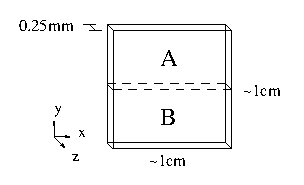
\includegraphics[width=2in]{mmi}
\label{fig:mmi}
\caption{Initial configuration of the MMI experiment for diffusively mixing solutions.}
\end{figure}
%%%%%%%%%%%%%%%%%%%%%%%%%%%%%%%%%

In our simulation we model a 0.8 cm $\times$ 0.8 cm $\times$ 0.25mm domain (very similar to the experimental
images shown over a 1.1 cm $\times$ 0.9 cm $\times$ 0.25mm domain).  We divide our domain into 
256 $\times$ 256 $\times$ 8 cubic grid cells.  We impose periodic boundary conditions in $x$,
a slip-reservoir boundary condition to match the initial configuration in $y$, and no-slip walls in $z$.
Gravity has a magnitude of 981cm/s$^2$ in the downward $y$ direction.  The characteristic velocities in
this simulation are sufficiently small that a diffusive CFL time step restriction needs to be imposed, i.e.,
$\Delta t = 6.39 \times 10^{-2}$s $= \sigma\Delta x^2/(2*d*D_{\rm max})$, with $\sigma=0.75$, 
dimensionality $d=3$, and $D_{\rm max}$ the maximum Maxwell-Stefan diffusion coefficient between any two pure
fluids.  We note that using this time step, the overdamped algorithm gives qualitatively
similar results by takes a factor of $\sim$4 more GMRES iterations to converge.  We use a limited trilinear
BDS advection scheme (Nonaka et al., J. Sci. Comput, 2011) and a viscous stress tensor formulation that 
ignores bulk viscosity effects.

The fluid parameters are $(\overline\rho_1, \overline\rho_2, \overline\rho_3) = (2.81, 1.55, 1.0)$ g/cm$^3$
with molecular masses of $(1.238\times 10^{-22}, 5.684\times 10^{-22}, 2.99\times 10^{-23})$ g/molecule.
The Maxwell-Stefan diffusion coefficients are
$D_{12} = 4.31826\times 10^{-6}, D_{13} = 1.91\times 10^{-5}$, and $D_{23} = 5.2\times 10^{-6}$.
We assume constant viscosity, $\eta = 0.01002$ P.  The initial mass fractions (concentrations) in the 
lower half of the domain are $c_{\rm lo} = (0, 0.1368, 0.8632)$ and in the upper half of the domain
are $c_{\rm hi} = (0.0864, 0, 0.9136)$.  This gives an initial density of 1.058932 g/cm$^3$ on top 
and 1.051018 g/cm$^3$ on bottom.  The ambient temperature is 293 K.

We perform two different simulations, both to $t\approx 63.9$ s (1000 time steps).
The first simulation uses a flat initial interface, but allows for thermal fluctuations in the mass
and momentum equations (we note that mass fluctuations are very small and do not cause any measureable
changes in any results).  The second simulation uses a randomly perturbed initial interface with one $xz$ plane 
of cells at the centerline randomly perturbed using $c = r c_{\rm lo} + (1-r) c_{\rm hi}$, with $r$ being a 
random number between 0.9 and 1.0 in each cell.  The scaling of this perturbation was chosen
so that the timescales of the pattern/spectra development match a flat initial interface with thermal fluctuations.

-Show figures of spectra for early time.  Comment how the 13 mm wavelength appears to be the dominant mode,
 as also reported by expterimentalists.

-Show images of structure development.


\section{Diffusive Layer Convection}
We modify the initial configuration of the MMI problem so we instead model
diffusive layer convection (DLC; see  Carballido-Landieira et al., Physics of Fluids, 2013).  
The setup remains similar to the MMI setup in that a salt-water solution sits on top
of a sucrose-water solution, but the concentrations of salt and sucrose solutes are modified 
so that we initially have a {\it light} salt-water solution ``A'' sitting upon a {\it heavier} 
sucrose-water solution ``B''.  We analyze the spectra of the vertically-averaged density, as 
is done in shadowgraph experiments.

As before, fluid ``1'' is salt solute, fluid ``2'' is sucrose solute, and fluid ``3'' is water.
The dimensions of the experiement are now 1 cm $\times$ 0.5 cm $\times$ 1 cm, with
periodic boundary conditions in $x$ and $z$, and a slip-reservoir boundary condition to match 
the initial configuration in $y$ (refer to Figure \ref{fig:dlc}).
The initial interface is either flat or slightly perturbed (depending on the simulation).
The buoyancy ratio between the two solutions combined with 
differential diffusion effects characterize this instability to be in the diffusive layer convection regime.
As in the MMI experiment, the rate at which the salt solute diffusives into pure water is $\sim$4 times greater 
than the rate at which the sucrose solute diffuses into water.
%%%%%%%%%%%%%%%%%%%%%%%%%%%%%%%%%
\begin{figure}[hb]
\centering
\includegraphics[width=2in]{dlc}
\label{fig:dlc}
\caption{Initial configuration of the DLC experiment for diffusively mixing solutions.}
\end{figure}
%%%%%%%%%%%%%%%%%%%%%%%%%%%%%%%%%

We divide our domain into 256 $\times$ 128 $\times$ 256 grid cells.  Gravity has a magnitude of 
981cm/s$^2$ in the downward $y$ direction.  We used a fixed time step of $\Delta t = 0.025$ s which
corresponds to an advective CFL of $\sigma\sim 0.5$.  We use an unlimited trilinear
BDS advection scheme (Nonaka et al., J. Sci. Comput, 2011) and a viscous stress tensor formulation that 
ignores bulk viscosity effects.  The fluid parameters are the same as the MMI experiement.
The initial mass fractions (concentrations) in the 
lower half of the domain are $c_{\rm lo} = (0, 0.05, 0.95)$ and in the upper half of the domain
are $c_{\rm hi} = (0.022, 0, 0.978)$.  This gives an initial density of 1.014375 g/cm$^3$ on top 
and 1.018062 g/cm$^3$ on bottom.  The ambient temperature is 293 K.

We perform two different simulations, both to $t=19$ s (760 time steps).
The first simulation uses a flat initial interface, but allows for thermal fluctuations in the mass
and momentum equations.  The second simulation uses a randomly perturbed initial interface with one $xz$ plane 
of cells at the centerline randomly perturbed using $c = r c_{\rm lo} + (1-r) c_{\rm hi}$, with $r$ being a 
random number between 0 and 1.0 in each cell.  The scaling of this perturbation was chosen
so that the timescales of the pattern/spectra development match a flat initial interface with thermal fluctuations.

Figure \ref{fig:dlc_images} illustrates vertically averaged densities and planar slices
of density for two different simulations.  The first simulation uses a randomly perturbed
initial interface without thermal fluctuations.  The second simulation uses a flat initial
interface with thermal fluctuations.  The vertical averaged densities are representative
of features visible using shadowgraph experimental techniques.
%%%%%%%%%%%%%%%%%%%%%%%%%%%%%%%%%
\begin{figure}[hb]
\centering
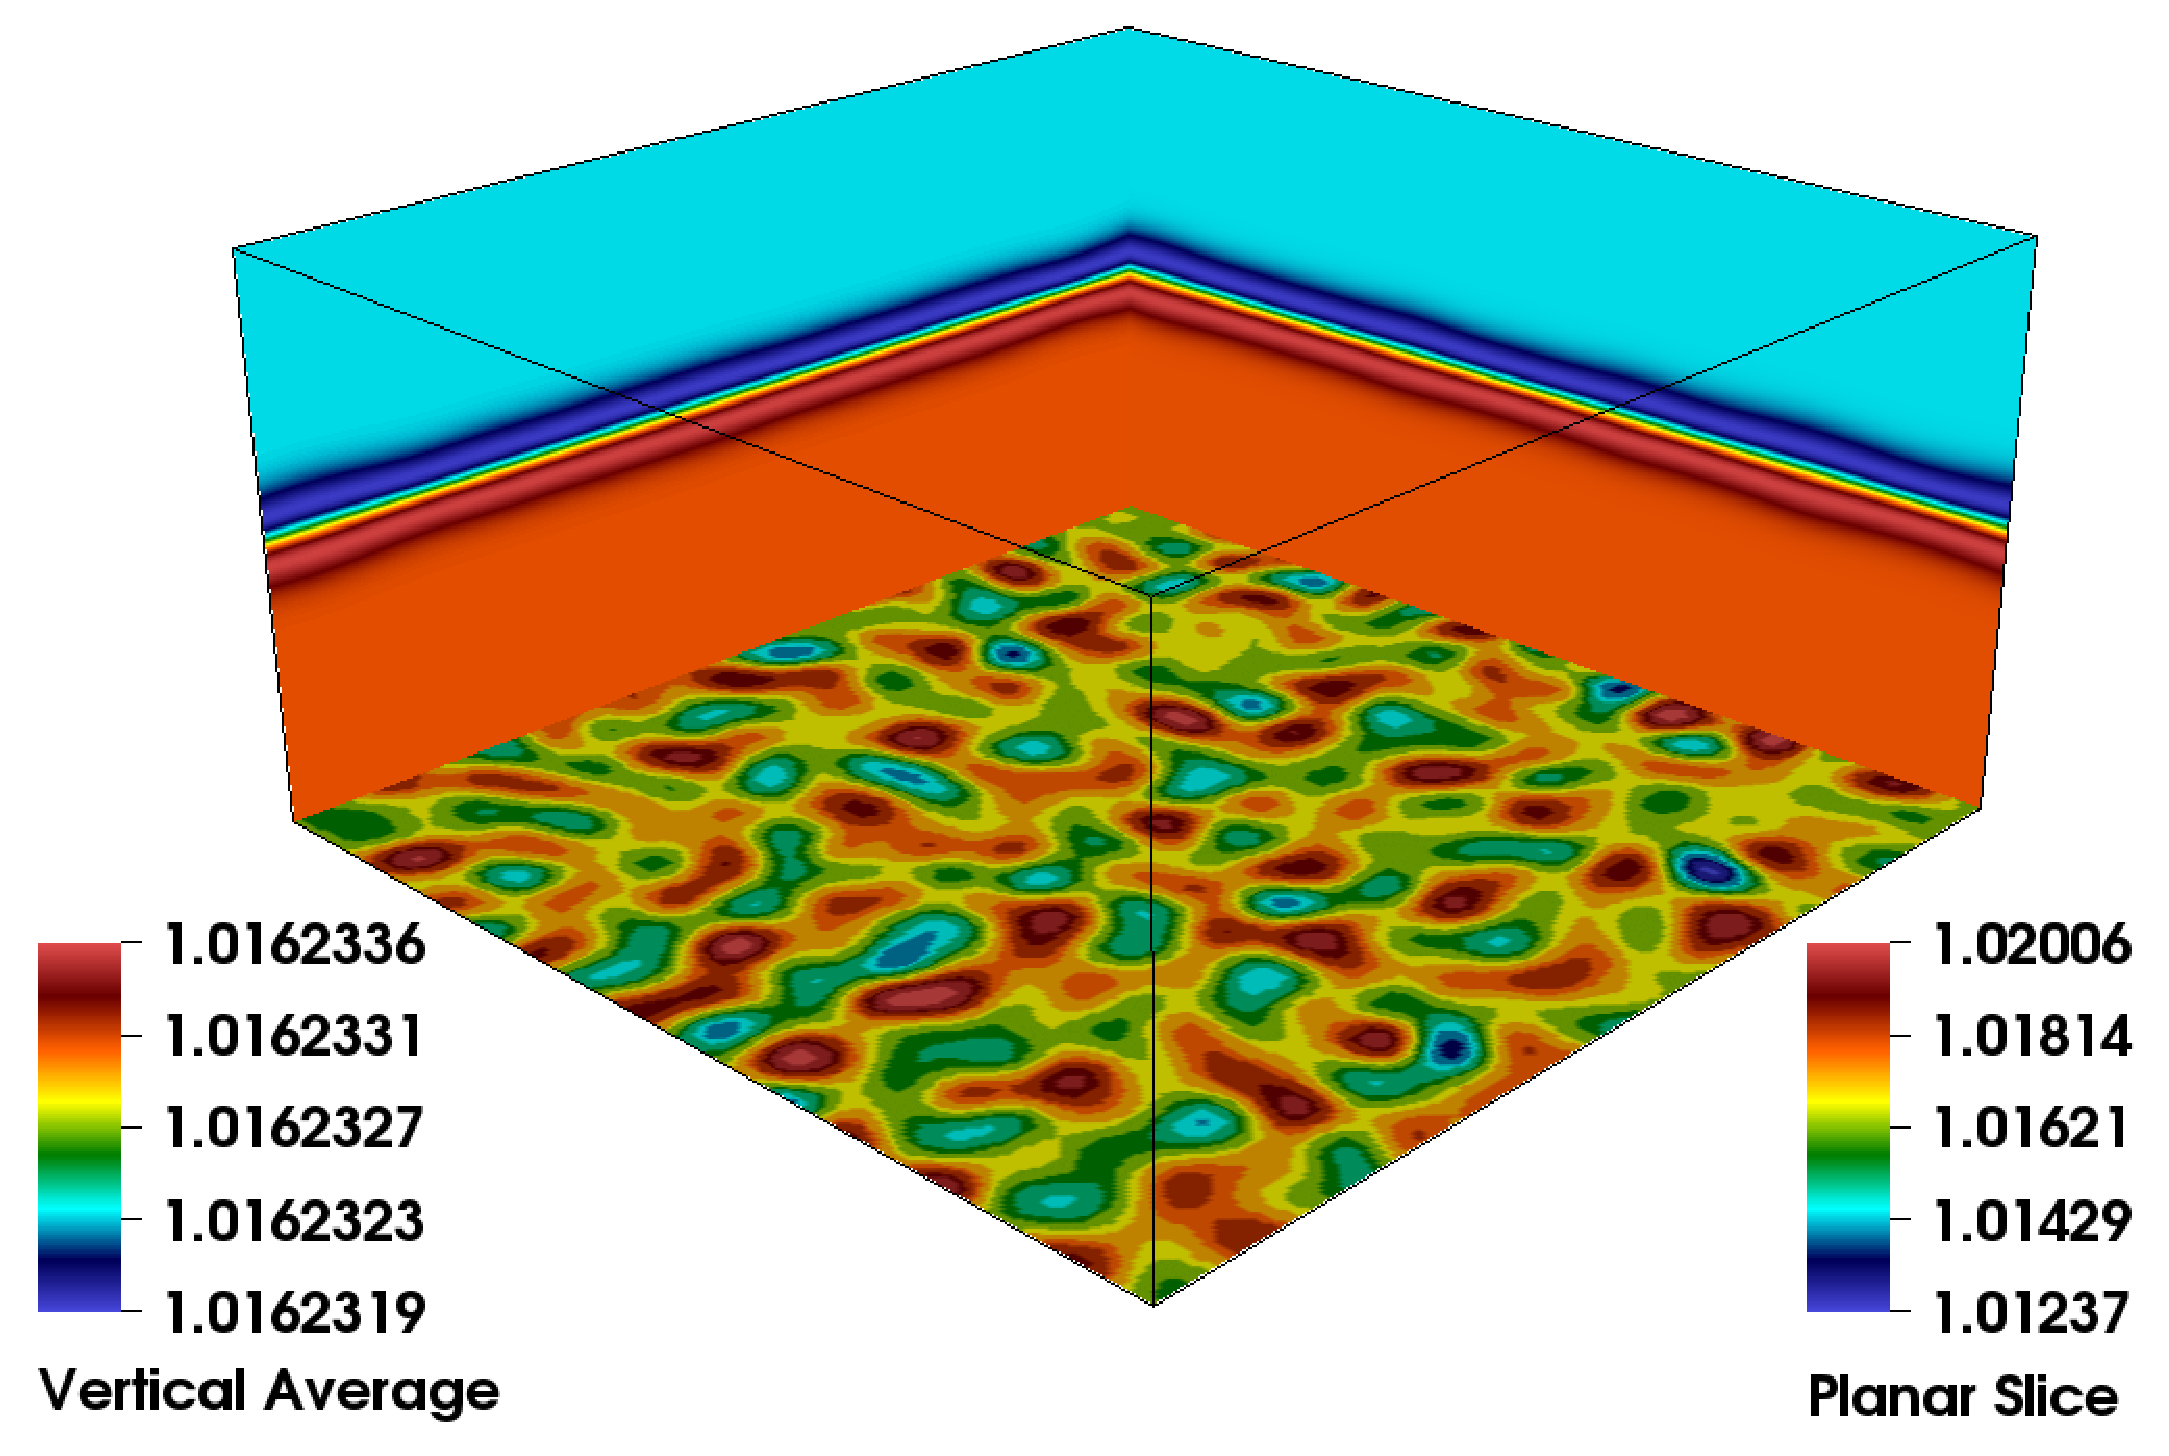
\includegraphics[width=2.75in]{DLC_pert_t15}
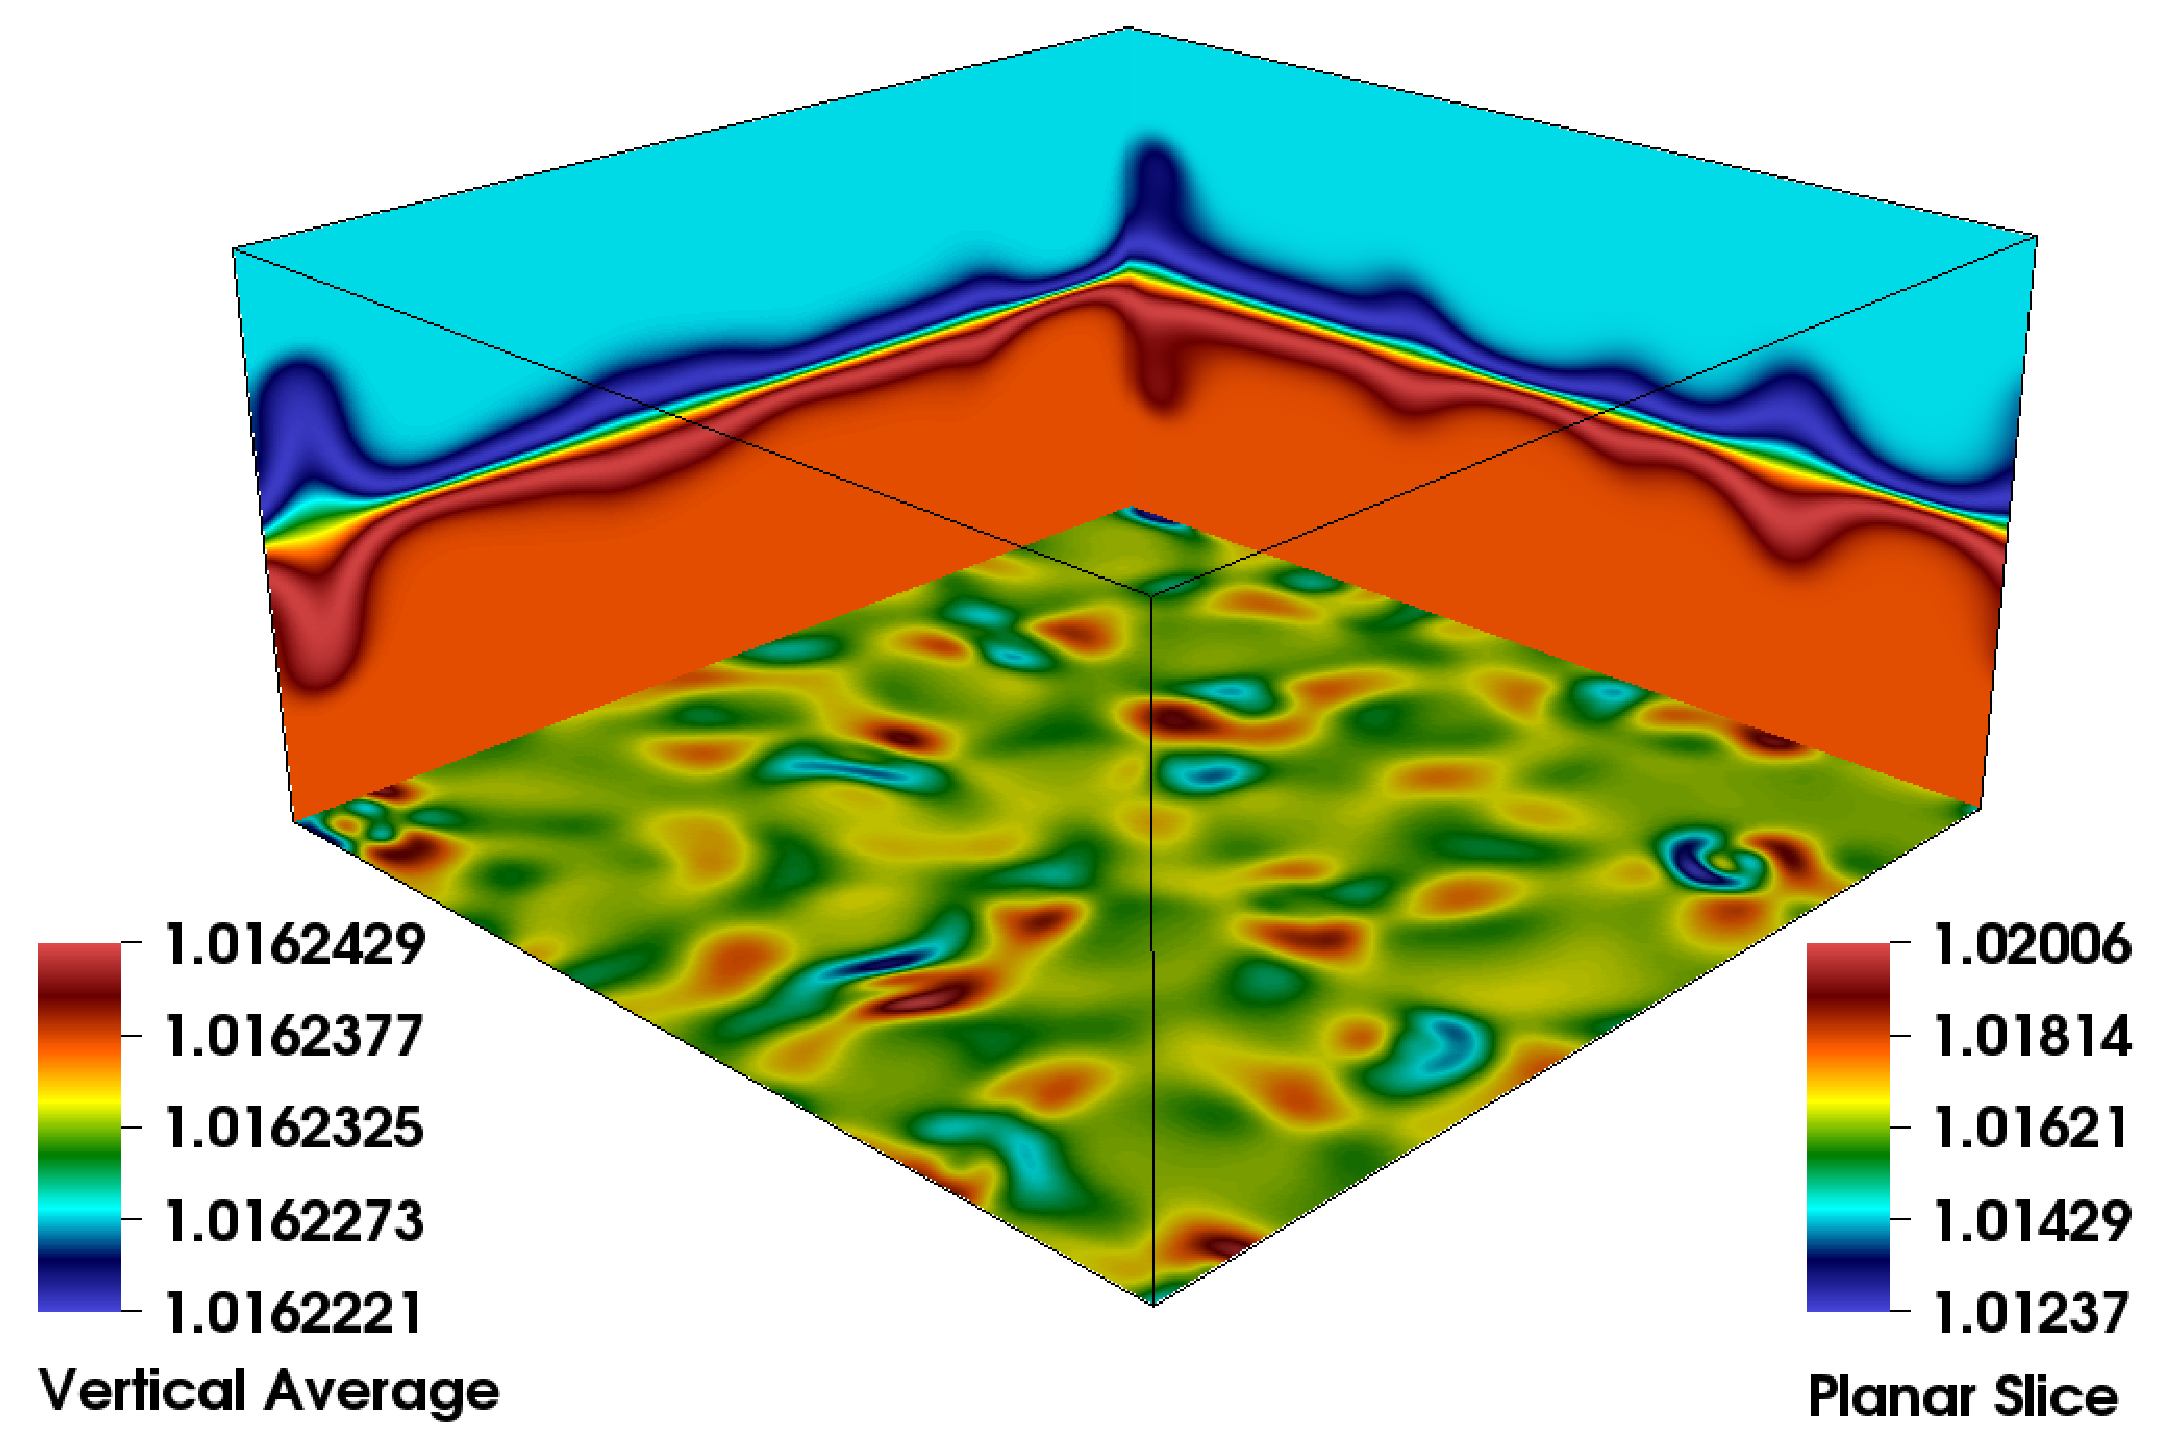
\includegraphics[width=2.75in]{DLC_pert_t19}\\
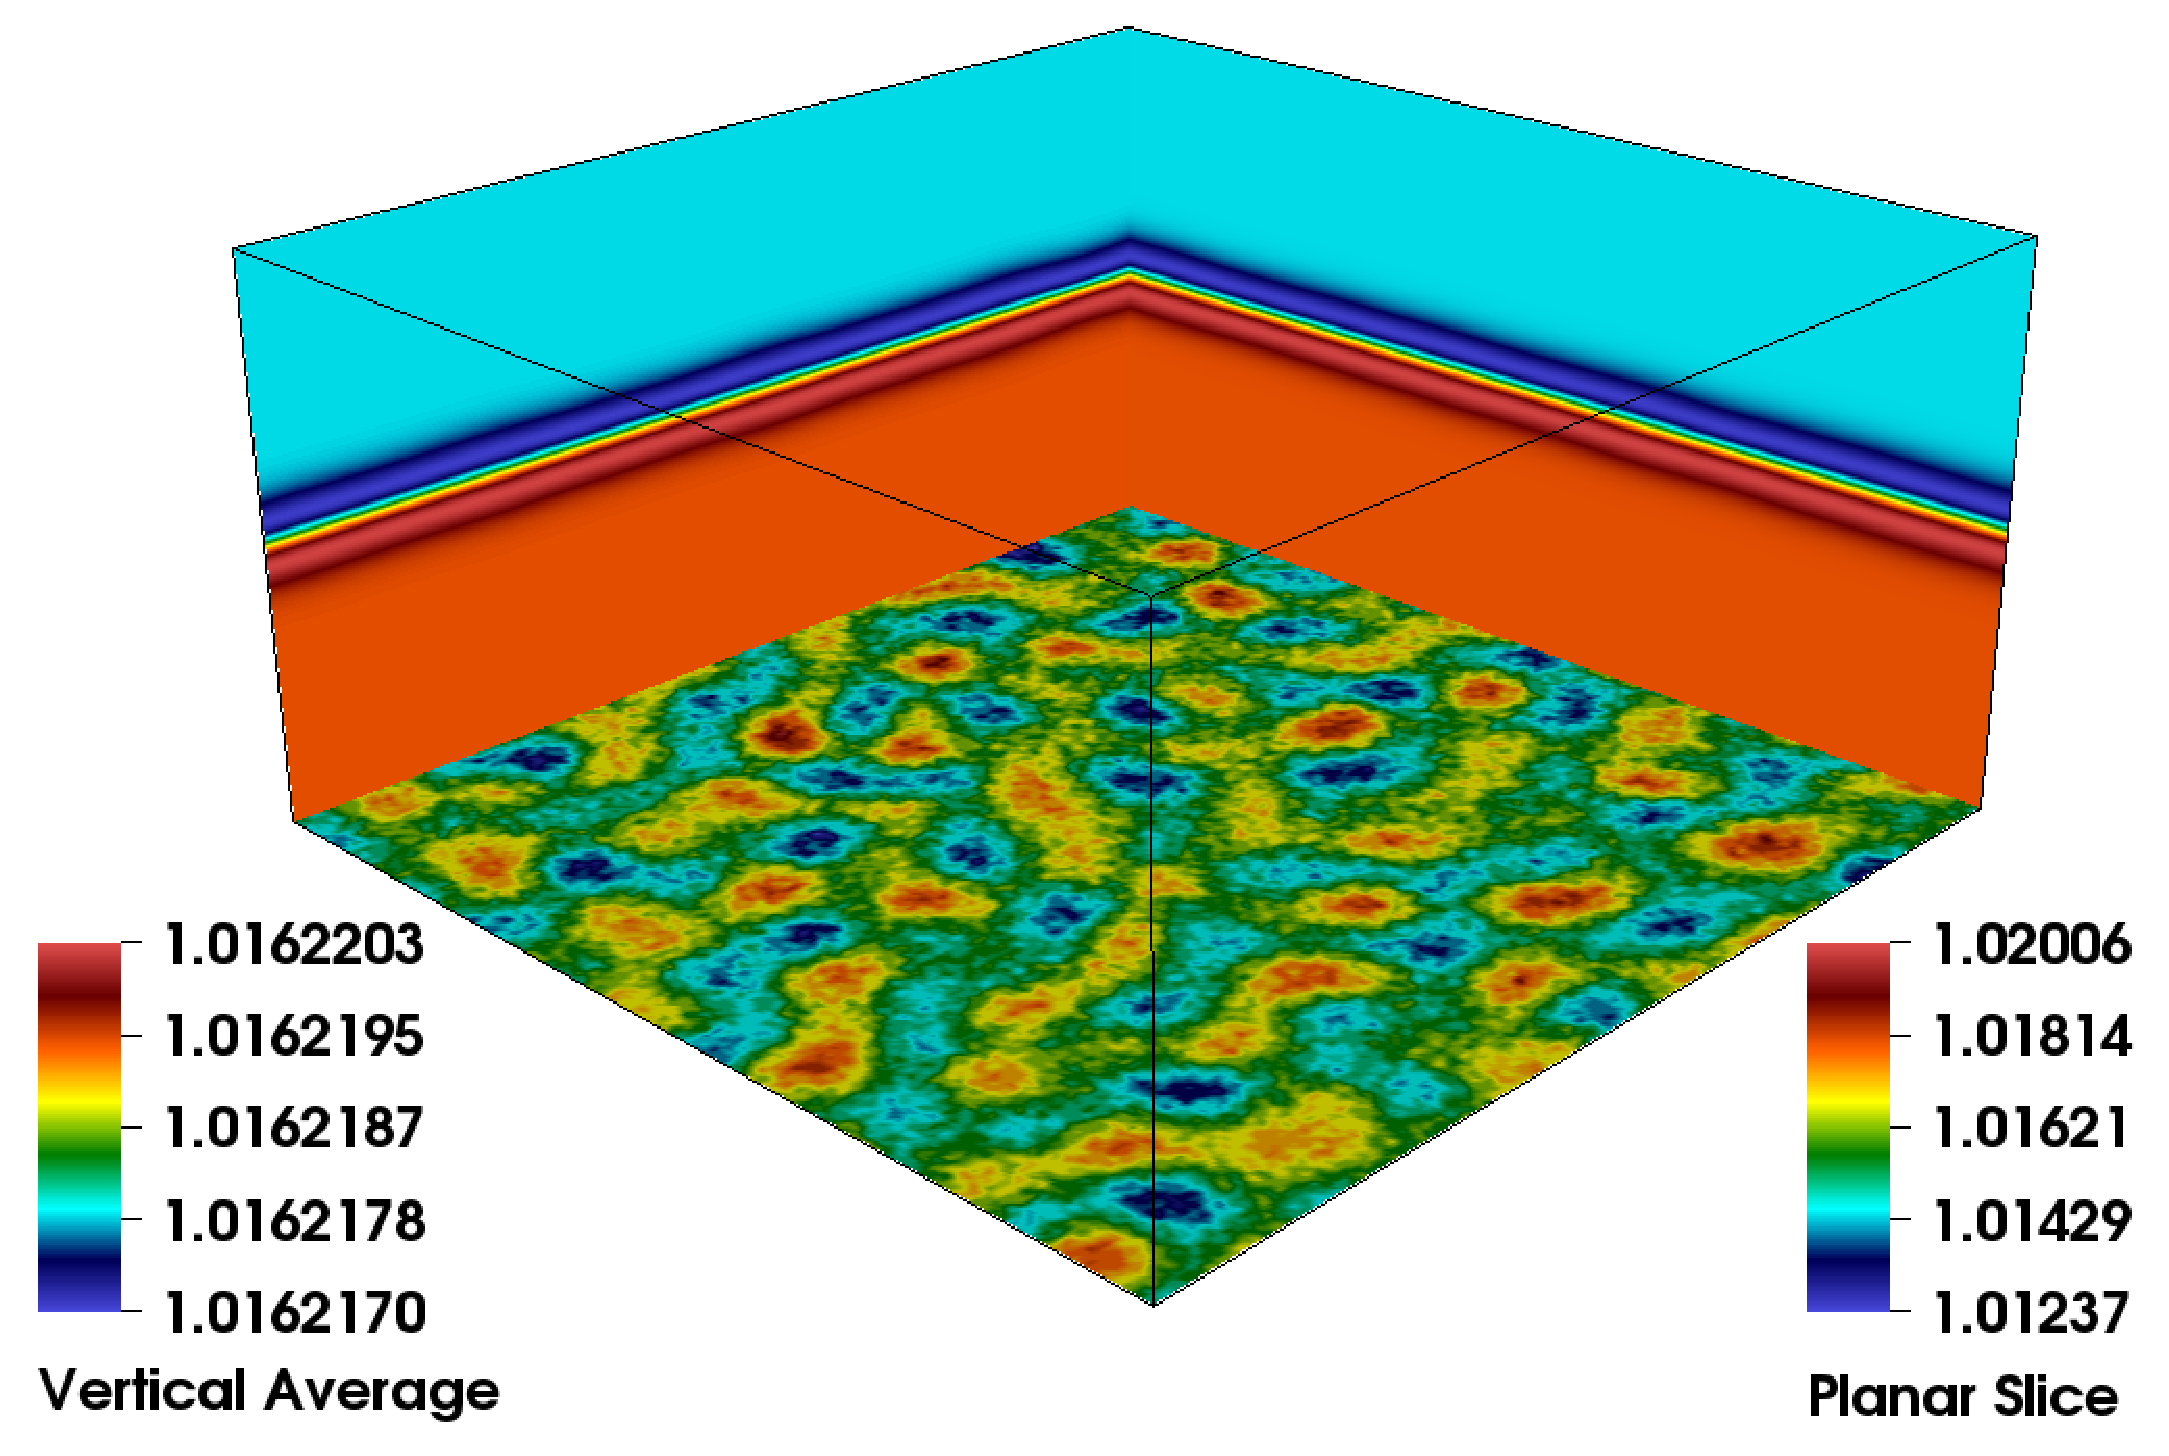
\includegraphics[width=2.75in]{DLC_therm_t15}
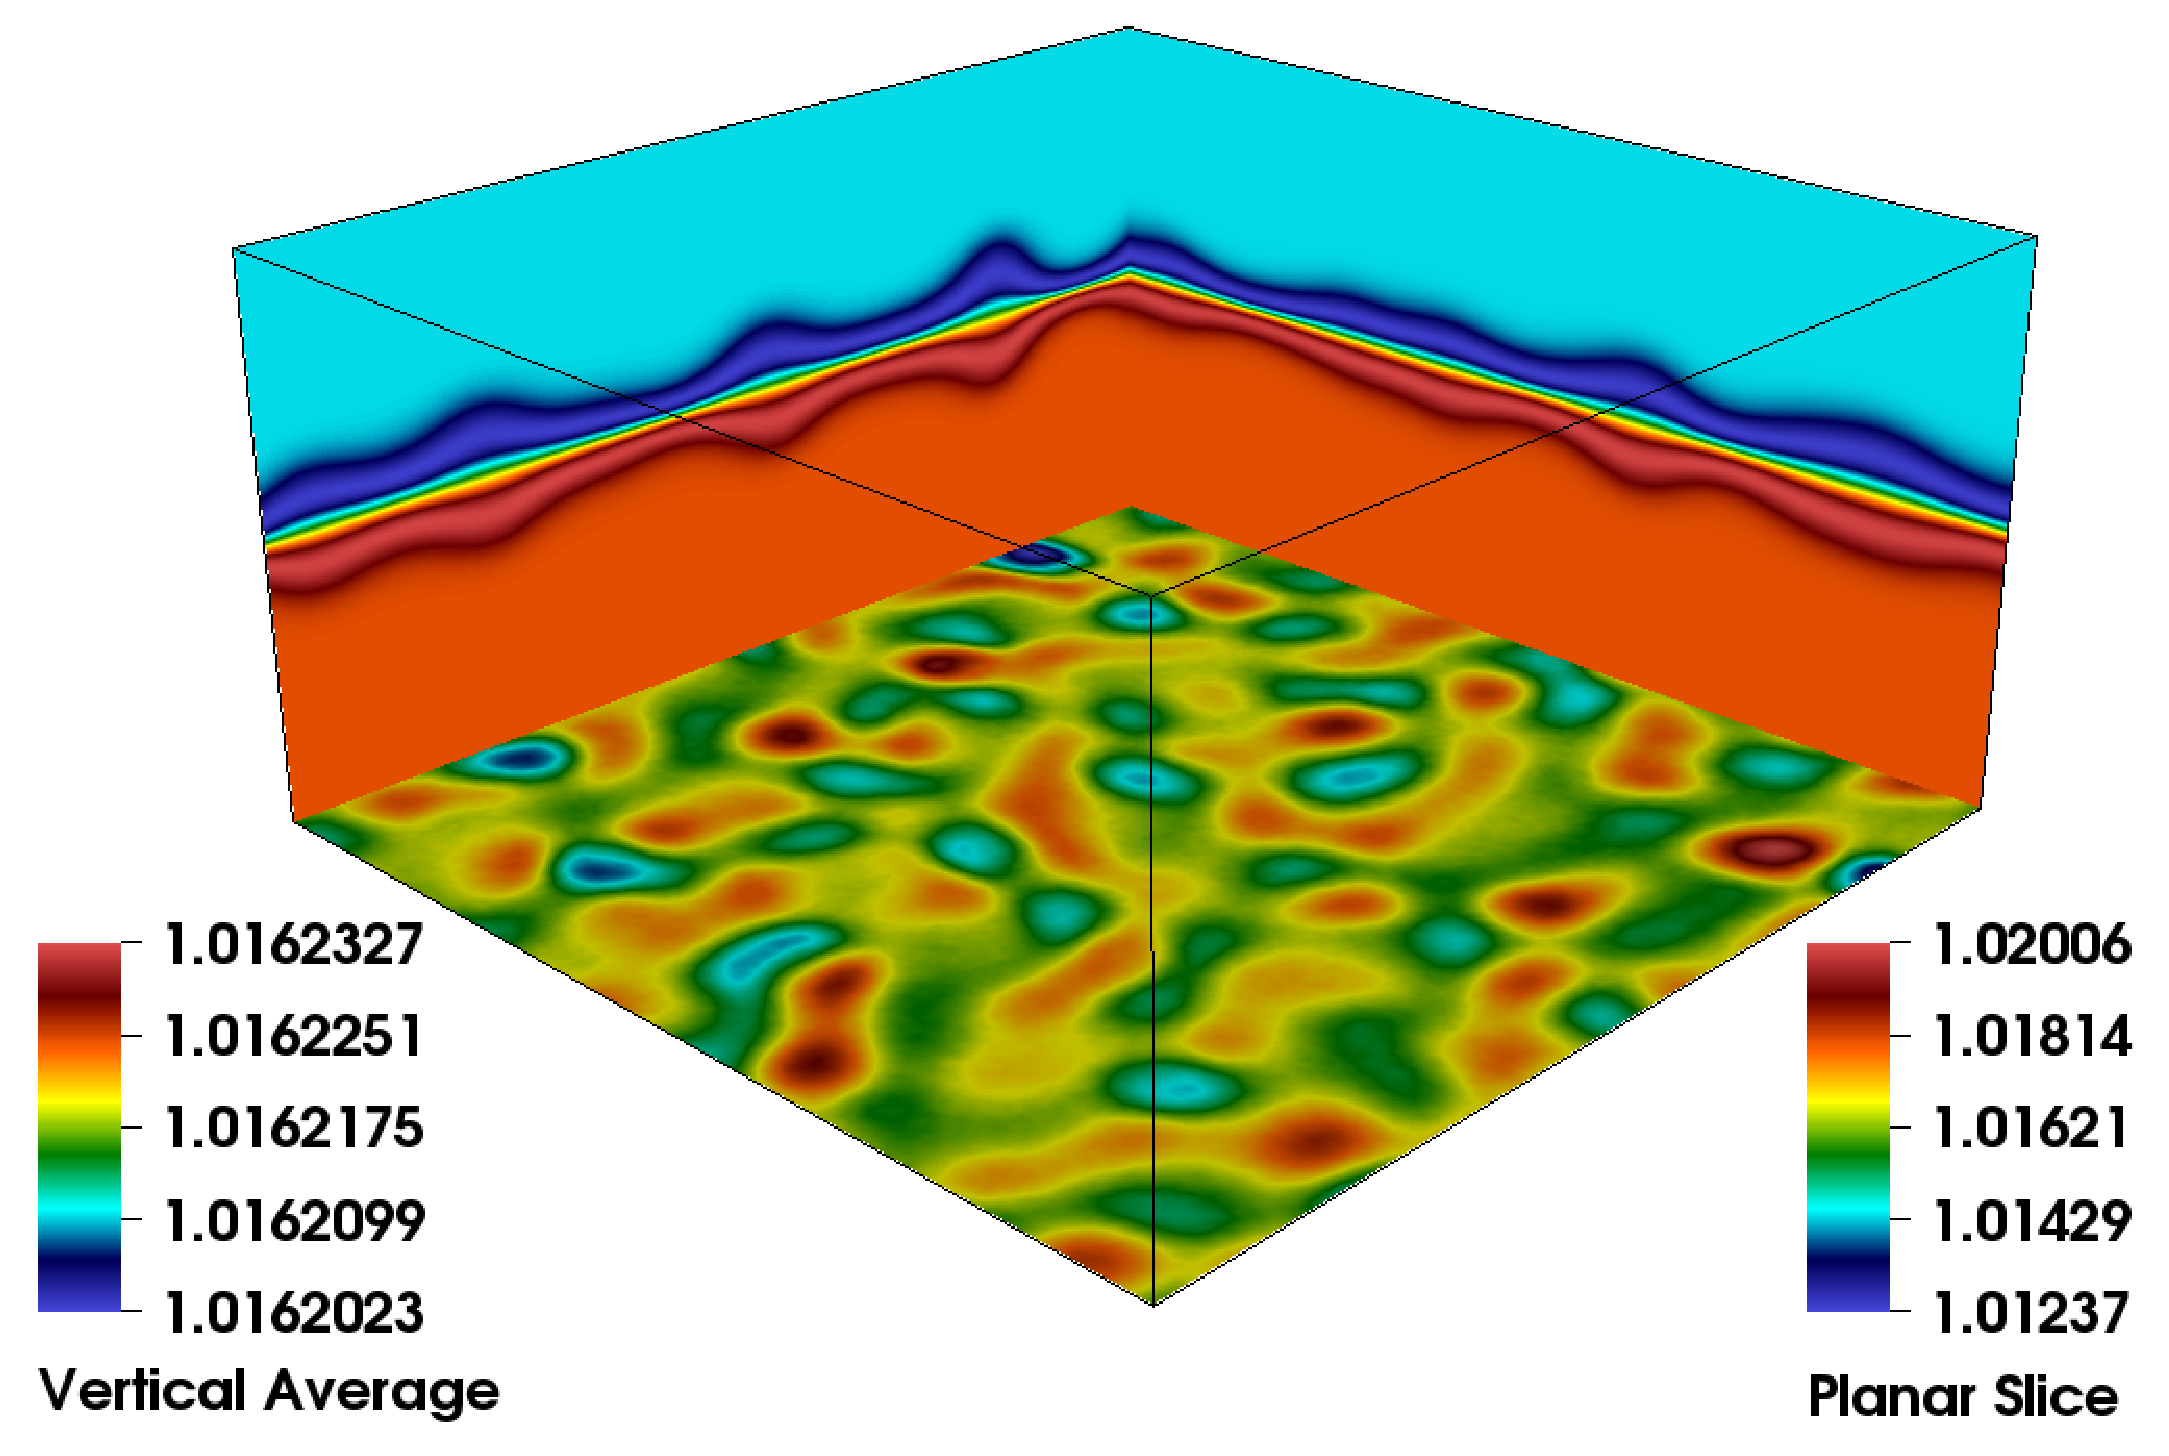
\includegraphics[width=2.75in]{DLC_therm_t19}
\label{fig:dlc_images}
\caption{Vertically averaged $\rho$ (illustrated on the $y$-planes) and planar
slices of $\rho$ ($x-$ and $z-$planes).  The top-left and top-right panes correspond
to $t=15$ and $19$ s from a simulation with a perturbed initial interface and no thermal
fluctuations.  The bottom-left and bottom-right panes correspond to $t=15$ and $19$ s
from a simulation with a flat initial interface with thermal fluctuations.}
\end{figure}
%%%%%%%%%%%%%%%%%%%%%%%%%%%%%%%%%

\section{2D Lid-Driven Cavity Convergence Testing}
The problem is a deterministic lid-driven cavity in two dimensions.
All units are cgs.
The domain is 1 $\times$ 1 divided into $64^2, 128^2, 256^2$, and $512^2$ grid cells.
The lo-y and hi-y walls are no-slip walls moving in equal and opposite directions,
setting up a circular flow pattern.  The hi-y wall speed is given by:
\begin{equation}
u(x,t) =
\begin{cases}
\frac{1}{4}\left[1 + \sin{(2\pi x - \frac{\pi}{2}})\right]
           \left[1 + \sin{(2\pi t - \frac{\pi}{2}})\right], & t < 0.5\\
\frac{1}{2}\left[1 + \sin{(2\pi x - \frac{\pi}{2}})\right], & t \ge 0.5
\end{cases}.
\end{equation}
The x-boundaries are stationary no-slip walls.
The time step for the coarsest simulation is $\Delta t=5\times 10^{-3}$ 
and is reduced by a factor of 2 as the resolution increases by a factor of 2.
This corresponds to an advective CFL number of $\sim 0.3$ for each simulation, and
a mass diffusion CFL of $\sim 0.67$ for the finest simulation.
We run each simulation to $t=2$.
We use $\bar\rho = (3,2,1)$.
The initial conditions are $\vb=0$ and $p=0$ with
a Gaussian bump of high density centered at $(x,y) = (0.5, 0.5)$ such that
\begin{eqnarray}
c_1 &=& 0.5e^{-75r^2}; \quad r = \sqrt{(x-0.5)^2 + (y-0.5)^2}, \\
c_2 &=& 0.5e^{-75r^2}, \\
c_3 &=& 1 - c_1 - c_2.
\end{eqnarray}
The viscosity varies linearly as a function of concentration, such that $\mu=0.1$
when $\rho=1$ and $\mu=1$ when $\rho=2.5$.  We use mass diffusion coefficients
$(D_{12},D_{13},D_{32}) = (10^{-4},5\times 10^{-4},10^{-3})$.
Gravity acts downward with $\gb=(0,-1)$, and we use
the viscous stress tensor formulation, $\taub = \eta[\nabla\vb + (\nabla\vb)^T]$.

In Table \ref{tab:Linf} we present convergence results in $L^\infty$ for the 
following test problems:
\begin{itemize}
\item Test 1: Inertial algorithm, centered scalar advection
\item Test 2: Inertial algorithm, unlimited bilinear BDS scalar advection.
\item Test 3: Inertial algorithm, unlimited quadratic BDS scalar advection.
\item Test 4: Inertial algorithm, unlimited bilinear BDS scalar advection, $\chi=0$.
\item Test 5: Overdamped algorithm, centered scalar advection
\item Test 6: Overdamped algorithm, unlimited bilinear BDS scalar advection.
\item Test 7: Overdamped algorithm, unlimited quadratic BDS scalar advection.
\item Test 8: Overdamped algorithm, unlimited bilinear BDS scalar advection, $\chi=0$.
\end{itemize}
%%%%%%%%%%%%%%%%%%%%%%%%%%%%%%%%%
\begin{table}[h]
\begin{center}
\caption{Refining in space and time.  Errors and convergence rates in $L^\infty$.}
\label{tab:Linf}
\begin{tabular}{ccccccc}
& & 64-128 & Rate & 128-256 & Rate & 256-512 \\
\hline
Test 1:             & $u$      & 1.83e-03 & 1.91 & 4.88e-04 & x.xx & x.xxe-xx \\
                    & $v$      & 7.01e-04 & 1.88 & 1.90e-04 & x.xx & x.xxe-xx \\
                    & $\rho_1$ & 4.04e-03 & 2.00 & 1.01e-03 & x.xx & x.xxe-xx \\
                    & $\rho_2$ & 3.97e-03 & 2.00 & 9.94e-04 & x.xx & x.xxe-xx \\
                    & $\rho_3$ & 3.33e-03 & 2.00 & 8.34e-04 & x.xx & x.xxe-xx \\
\hline
Test 2:             & $u$      & x.xxe-xx & x.xx & x.xxe-xx & x.xx & x.xxe-xx \\
                    & $v$      & x.xxe-xx & x.xx & x.xxe-xx & x.xx & x.xxe-xx \\
                    & $\rho_1$ & x.xxe-xx & x.xx & x.xxe-xx & x.xx & x.xxe-xx \\
                    & $\rho_2$ & x.xxe-xx & x.xx & x.xxe-xx & x.xx & x.xxe-xx \\
                    & $\rho_3$ & x.xxe-xx & x.xx & x.xxe-xx & x.xx & x.xxe-xx \\
\hline
Test 3:             & $u$      & x.xxe-xx & x.xx & x.xxe-xx & x.xx & x.xxe-xx \\
                    & $v$      & x.xxe-xx & x.xx & x.xxe-xx & x.xx & x.xxe-xx \\
                    & $\rho_1$ & x.xxe-xx & x.xx & x.xxe-xx & x.xx & x.xxe-xx \\
                    & $\rho_2$ & x.xxe-xx & x.xx & x.xxe-xx & x.xx & x.xxe-xx \\
                    & $\rho_3$ & x.xxe-xx & x.xx & x.xxe-xx & x.xx & x.xxe-xx \\
\hline
Test 4:             & $u$      & x.xxe-xx & x.xx & x.xxe-xx & x.xx & x.xxe-xx \\
                    & $v$      & x.xxe-xx & x.xx & x.xxe-xx & x.xx & x.xxe-xx \\
                    & $\rho_1$ & x.xxe-xx & x.xx & x.xxe-xx & x.xx & x.xxe-xx \\
                    & $\rho_2$ & x.xxe-xx & x.xx & x.xxe-xx & x.xx & x.xxe-xx \\
                    & $\rho_3$ & x.xxe-xx & x.xx & x.xxe-xx & x.xx & x.xxe-xx \\
\hline
Test 5:             & $\rho_1$ & x.xxe-xx & x.xx & x.xxe-xx & x.xx & x.xxe-xx \\
                    & $\rho_2$ & x.xxe-xx & x.xx & x.xxe-xx & x.xx & x.xxe-xx \\
                    & $\rho_3$ & x.xxe-xx & x.xx & x.xxe-xx & x.xx & x.xxe-xx \\
\hline
Test 6:             & $\rho_1$ & x.xxe-xx & x.xx & x.xxe-xx & x.xx & x.xxe-xx \\
                    & $\rho_2$ & x.xxe-xx & x.xx & x.xxe-xx & x.xx & x.xxe-xx \\
                    & $\rho_3$ & x.xxe-xx & x.xx & x.xxe-xx & x.xx & x.xxe-xx \\
\hline
Test 7:             & $\rho_1$ & x.xxe-xx & x.xx & x.xxe-xx & x.xx & x.xxe-xx \\
                    & $\rho_2$ & x.xxe-xx & x.xx & x.xxe-xx & x.xx & x.xxe-xx \\
                    & $\rho_3$ & x.xxe-xx & x.xx & x.xxe-xx & x.xx & x.xxe-xx \\
\hline
Test 8:             & $\rho_1$ & x.xxe-xx & x.xx & x.xxe-xx & x.xx & x.xxe-xx \\
                    & $\rho_2$ & x.xxe-xx & x.xx & x.xxe-xx & x.xx & x.xxe-xx \\
                    & $\rho_3$ & x.xxe-xx & x.xx & x.xxe-xx & x.xx & x.xxe-xx
\end{tabular}
\end{center}
\end{table}
%%%%%%%%%%%%%%%%%%%%%%%%%%%%%%%%%

\end{document}
